\chapter{Prediction Evaluation}\label{prediction_evaluation}

	\maheshi{This currently only mentions the Edinburgh data set as that's all I have for now.}

	\section{Motivation}\label{prediction_evaluation_motivation}

		In sampling data it is almost inevitable that information will be missed. In order to accurately reconstruct the original data we must take certain precautions. One of these precautions is making sure that we sample at a rate high enough to reconstruct all information. This rate goes by the term \emph{Nyquist rate}~\cite{nyquistrate}. The Nyquist rate is the rate of taking measurements such that the original information can be reconstructed without aliasing occurring. This essentially means that we need to have a sample rate of twice the rate of the smallest changes in a signal. If we do not have this sampling rate then it is possible for us to lose information during the sampling process. 

		\centerimagewideanywhere{./images/Nyquist_Example.png}{Here we can see an example of a sample rate on the function $y = sin(4x)$ being insufficient. This sample rate of 1.2 is insufficient for the graph since it's period is $\frac{2\pi}{4} \equiv 1.570$. A sample rate of $\frac{1.570}{2} \equiv 0.785$ is required to be sufficient.}{fig:nyquist_example}

		When measuring air quality we almost certainly will not meet the Nyquist rate and therefore need to compensate. Without any interpolation or extrapolation methods the best we can do is generate data similar to that seen in figure~\ref{fig:stationarypollutantbuildup}. In this figure we see that we only have information where pollutants were measured. In this case it was done with a sensor on a bus and therefore limited to the roads. 

		\centerimagewideanywhere{./images/StationaryPollutantBuildUp.png}{A map of air pollution around Edinburgh city centre. Image uses \emph{Open Street Map}.}{fig:stationarypollutantbuildup}

		\centerimageanywhere{.5\textwidth}{./images/zurichpm.jpg}{A heatmap of particulate matter in Zurich. The higher pollution levels can clearly be seen to follow transport infrastructure.~\cite{opensensezurich}}{fig:zurichheatmap}

		The solution is to interpolate and extrapolate our data so that what we see in figure~\ref{fig:stationarypollutantbuildup} can be converted into something similar to figure~\ref{fig:zurichheatmap}, where we have estimations of pollutant levels in areas where we did not take measurements. 

		With air quality data, many institutes and organisations use complex methods of interpolating the data such as \emph{Land Use Regression (LUR)}~\cite{lurtraffic}. LUR and other advanced models~\cite{reviewofaqmodels} have advantages over simple interpolation models in that they can take information about the sampling environment into account. By providing this auxiliary information, such as known sources of pollution, terrain, buildings, etc. we can greatly improve the accuracy of the estimations that these advanced models produce. These models are not without their disadvantages however. One of the main drawbacks of these are the considerably complexity of development and use. As such it would be useful to determine if simple interpolation algorithms, such as those designed for image or sound processing, are effective at interpolation air quality data sets. The algorithms which will be tested are those discussed in section~\ref{background_interpolation_methods}. These algorithms are: 

		\begin{itemize}
	        \item Bilinear interpolation
	        \item Bicubic interpolation
	        \item Natural neighbour interpolation
	        \item Barnes interpolation
	        \item Nearest neighbour interpolation
	        \item Inverse distance weighting interpolation
	    \end{itemize}

	    The bilinear and bicubic algorithms are generally used for interpolating pixels in images when resized. Natural neighbour, nearest neighbour and inverse distance weighted are more generic interpolation algorithms, and Barnes interpolation has seen application in weather forecasting~\cite{barnesinterpolation}. These applications were chosen as all are commonly used and are simple to understand. 



	\section{Methodology}\label{prediction_evaluation_methodology}

		In order to evaluate the efficiency of these algorithms we will utilise an existing data set of air quality measurements. The initial step is to remove some known values from our data set. If we then apply the various interpolation algorithms to this data set, then we will have predicted values at the points which we removed. By comparing these predicted values and the actual values recorded we will have a metric for comparing the efficiency of the various algorithms. 

		\subsection{Data Sets}\label{prediction_evaluation_methodology_data_sets}

			\subsubsection{OpenSense}\label{prediction_evaluation_methodology_data_sets_opensense}

				\maheshi{Still waiting on this data set.}

				This data set, provided by the \emph{OpenSense} group at \emph{ETH Zurich}, provides ozone concentrations based on measurements taken from trams moving around the city of Zurich, Switzerland. This data set only has measurements along the tram tracks, similar to how data would only be provided along bus routes with a physical implementation of this system. We will perform our interpolation on the entire data set giving a two dimensional map covering the city of estimated ozone concentrations. We will then use information taken from static sensors located in Zurich, which are not along tram tracks, to measure the accuracy of these interpolation algorithms. 

				\centerimagewideanywhere{./images/Zurich_Ozone.png}{A scatter plot of the Zurich data points. The hue of the colour of the points is directly proportional to the Ozone concentration.}{fig:zurich_ozone}

				While this data set is the most realistic in terms of mimicking the data from buses around Edinburgh, it does pose certain problems. The foremost of these is that there are only two static sensors which we can use to determine the accuracy of our algorithms. Two sensors is enough to show whether some algorithms perform better than others within some degree of certainty, but does not give information about the absolute accuracy of the algorithms. 

				A second problem, is one which affects all data sets we would use. That is the issues caused by the temporal changes in the data. If we were to take the measurements at any given point in time we would only have as many data points as there are sensors, which may not provide sufficient coverage. We can assume that pollutant levels do not change so quickly in that we would have extreme differences between readings. By making this assumption we can select a temporal window of measurements and so can increase the number of readings we have. These readings will also be at different locations due to the motion of the trams, giving a better representation of the actual data, and in so improving the accuracy of our algorithms. 

				In taking this temporal window we risk missing out on some information. Should a pollutant change rapidly in the space of a single window, this information would be lost, and may indeed skew the results. Experimentation revealed that a window of 30 minutes is enough to cover as much area as possible, with minimal overlap of tram routes. \todo{Still not happy about this. I should show this somehow. }


			\subsubsection{Air Quality Scotland}\label{prediction_evaluation_methodology_data_sets_air_quality_scotland}

				The data set from \emph{Air Quality Scotland} is much simpler, and therefore less useful, than the OpenSense data set. This data set consists of eight static air quality monitoring stations across Edinburgh. Out of these eight stations, five form the convex hull of the data set, and one of the internal stations is in a high traffic zone. The result of this is that we only have three points which we can use to check our calculations, and one of these is going to have a large discrepancy between the actual values and the estimated values. Furthermore, this data set only has the means at one hour intervals and so the temporal drift mentioned in the above section still applies. However, one advantage that this data set does provide is three different chemical readings to use. 

		\subsection{Data Structure}\label{prediction_evaluation_methodology_data_structure}
			
			In order to use these data sets in the various algorithms we must change the data structure slightly. Two of the algorithms, bilinear interpolation, and bilinear interpolation, work when the data is on a regular grid, which these data sets are not. As such we need to map them onto a regular grid. For the algorithms which are not limited to a grid we do not have to

			With the Zurich data set the area which we are taking measurements from is roughly $5km$ by $5km$. By setting a resolution of 200 by 200 for the grid we can calculate the interpolated values in regions roughly $25m$ by $25m$. Using the same resolution on the Edinburgh data we move our data points from a map of size $15km$ by $9km$ to a grid with cells of size $75m$ by $45m$. These resolutions can be deemed as high resolution~\cite{spatiotemporalresolution}.


    \section{Results}\label{prediction_evaluation_results}

        \subsection{Nearest Neighbour}\label{prediction_evaluation_results_nearest_neighbour}

	        \centerimagewide{./images/Nearest_Neighbour_Zurich.png}{The result of applying the nearest neighbour algorithm to the data seen in figure~\ref{fig:zurich_ozone}.}{fig:nearest_neighbour_zurich}

	        The nearest neighbour algorithm is our simplest interpolation method, and due to that it almost acts as a baseline to compare to. We would expect this algorithm to have the worst performance on most data sets. When we apply the nearest neighbour algorithm to the data set seen in figure~\ref{fig:zurich_ozone} we get a result similar to that seen in figure~\ref{fig:nearest_neighbour_zurich}. When we apply it to the Edinburgh data set we get results seen in figure~\ref{fig:nearest_neighbour_difference_results}. 

	        \iffalse
		        \begin{table}[H]
		        	\centering
		    		\begin{tabular}{|c|c|c|c|c|c|c|}
		    			\hline
				        Pollutant & Time & Actual & Estimated & Difference & Absolute Difference & Difference (\%) \\ \hline
						$NO$ & 1 & 19.00 & 20.67 & 1.67 & 1.67 & 8.77 \\
						$NO$ & 2 & 10.67 & 10.00 & -0.67 & 0.67 & 6.25 \\
						$NO$ & 3 & 26.00 & 12.33 & -13.67 & 13.67 & 52.56 \\
						$NO$ & 4 & 17.00 & 12.33 & -4.67 & 4.67 & 27.45 \\
						$NO$ & 5 & 33.00 & 20.67 & -12.33 & 12.33 & 37.37 \\
						$NO$ & 6 & 42.00 & 37.00 & -5.00 & 5.00 & 11.90 \\
						$NO$ & 7 & 138.00 & 97.67 & -40.33 & 40.33 & 29.23 \\
						$NO$ & 8 & 226.00 & 186.67 & -39.33 & 39.33 & 17.40 \\
						$NO_{2}$ & 1 & 40.67 & 41.33 & 0.67 & 0.67 & 1.64 \\
						$NO_{2}$ & 2 & 39.00 & 40.67 & 1.67 & 1.67 & 4.27 \\
						$NO_{2}$ & 3 & 42.00 & 42.67 & 0.67 & 0.67 & 1.59 \\
						$NO_{2}$ & 4 & 42.00 & 41.00 & -1.00 & 1.00 & 2.38 \\
						$NO_{2}$ & 5 & 42.33 & 39.00 & -3.33 & 3.33 & 7.87 \\
						$NO_{2}$ & 6 & 44.67 & 45.33 & 0.67 & 0.67 & 1.49 \\
						$NO_{2}$ & 7 & 63.00 & 66.33 & 3.33 & 3.33 & 5.29 \\
						$NO_{2}$ & 8 & 85.67 & 90.33 & 4.67 & 4.67 & 5.45 \\
						$NO_{X}$ & 1 & 70.00 & 73.33 & 3.33 & 3.33 & 4.76 \\
						$NO_{X}$ & 2 & 55.67 & 56.33 & 0.67 & 0.67 & 1.20 \\
						$NO_{X}$ & 3 & 82.33 & 61.67 & -20.67 & 20.67 & 25.10 \\
						$NO_{X}$ & 4 & 68.33 & 60.00 & -8.33 & 8.33 & 12.20 \\
						$NO_{X}$ & 5 & 93.00 & 70.67 & -22.33 & 22.33 & 24.01 \\
						$NO_{X}$ & 6 & 108.67 & 101.67 & -7.00 & 7.00 & 6.44 \\
						$NO_{X}$ & 7 & 274.67 & 216.00 & -58.67 & 58.67 & 21.36 \\
						$NO_{X}$ & 8 & 431.67 & 376.33 & -55.33 & 55.33 & 12.82 \\ \hline
					\end{tabular}
					\caption{The results of running the nearest neighbour algorithm, averaged across three different measurement points.}
					\label{tab:nearest_neighbour_difference_results}
				\end{table}
			\fi

			\centerimagewide{./images/Nearest_Neighbour_Percentage_Differences.png}{The results of running the nearest neighbour algorithm as a scatter plot, averaged across three different measurement points.}{fig:nearest_neighbour_difference_results}

			From this scatter plot we get the first information about our interpolation algorithm. Initially we can see that $NO_{2}$ has a much lower percentage difference on average than the other pollutants. We can also see that there seems to be some correlation between the percentage difference of the value of $NO$ and the value of $NO_{X}$. 

			In order to have a metric which allows us to evaluate the performance we must take the mean of the deviation across all time periods. Further research concluded that using the root mean square is the standard method of assessing the accuracy of air pollution models~\cite{spatiotemporalresolution}, however, due to the fact that the remaining sections use the mean deviation method and that they are compared relative to each other, this is not an issue. This data is shown in table~\ref{tab:nearest_neighbour_difference_results_mean}. 

			\begin{table}[H]
				\centering
	    		\begin{tabular}{|c|c|}
	    			\hline
			        Pollutant & Difference (\%) \\ \hline
					$NO$ & 23.87 \\
					$NO_{2}$ & 3.75 \\
					$NO_{X}$ & 13.49 \\ \hline
				\end{tabular}
				\caption{The mean results of the data in figure~\ref{fig:nearest_neighbour_difference_results}.}
				\label{tab:nearest_neighbour_difference_results_mean}
			\end{table}

		\subsection{Nearest Neighbour with Convolution Filter}\label{prediction_evaluation_results_nearest_neighbour_convolution_filter}

			\centerimagewide{./images/Nearest_Neighbour_Sigma_6_Zurich.png}{The result of applying the nearest neighbour with convolution filter algorithm to the data seen in figure~\ref{fig:zurich_ozone}. This is the result of setting $\sigma$ to the value of 6.}{fig:nearest_neighbour_blur_zurich}

			As was mentioned in section~\ref{background_interpolation_methods_nearest_neighbour}, a possible optimisation to the nearest neighbour algorithm is to apply a convolution filter to it. In this case we will use a Gaussian blur as our convolution filter. The formula for applying a Gaussian blur in two dimension~\cite{gaussianblur} is:

			\begin{align*}
				G(x,y) = \frac{1}{2\pi\sigma^{2}} e^{-\frac{x^{2} + y^{2}}{2\sigma^{2}}}
			\end{align*}

			As we can see from this equation, we have introduced a new parameter $\sigma$. In order to evaluate the effectiveness of this algorithm we must also have an optimal value of $\sigma$. To find this optimal value, the tests were run the same way as they were in the previous section, but this time we also had $\sigma$ as a variable. By taking the mean of the results across all time frames and plotting this against the value of sigma, our results are that of figure~\ref{fig:nearest_neighbour_convolution_sigma_results}. 

			\iffalse
				\begin{table}[H]
					\centering
		    		\begin{tabular}{|c|c|c|c|c|c|c|}
		    			\hline
						Pollutant & Sigma & Difference \\ \hline
						$NO$ & 1 & 202.40 \\
						$NO$ & 2 & 200.90 \\
						$NO$ & 4 & 189.34 \\
						$NO$ & 8 & 182.73 \\
						$NO$ & 16 & 189.79 \\
						$NO$ & 32 & 187.60 \\
						$NO$ & 64 & 174.09 \\
						$NO$ & 128 & 166.21 \\
						$NO$ & 256 & 163.23 \\
						$NO$ & 512 & 163.22 \\
						$NO_{2}$ & 1 & 167.43 \\
						$NO_{2}$ & 2 & 166.80 \\
						$NO_{2}$ & 4 & 157.71 \\
						$NO_{2}$ & 8 & 147.90 \\
						$NO_{2}$ & 16 & 145.19 \\
						$NO_{2}$ & 32 & 144.66 \\
						$NO_{2}$ & 64 & 133.29 \\
						$NO_{2}$ & 128 & 127.46 \\
						$NO_{2}$ & 256 & 126.20 \\
						$NO_{2}$ & 512 & 126.20 \\
						$NO_{x}$ & 1 & 166.89 \\
						$NO_{x}$ & 2 & 166.13 \\
						$NO_{x}$ & 4 & 156.69 \\
						$NO_{x}$ & 8 & 146.44 \\
						$NO_{x}$ & 16 & 143.22 \\
						$NO_{x}$ & 32 & 142.87 \\
						$NO_{x}$ & 64 & 132.21 \\
						$NO_{x}$ & 128 & 126.95 \\
						$NO_{x}$ & 256 & 125.87 \\
						$NO_{x}$ & 512 & 125.87 \\ \hline
					\end{tabular}
					\caption{The mean results of varying the value of $\sigma$ in applying a Gaussian blur to the nearest neighbour results.}
					\label{tab:nearest_neighbour_convolution_sigma_results}
				\end{table}
			\fi

			\centerimagewide{./images/Nearest_Neighbour_Gaussian_Blur.png}{The mean results of varying the value of $\sigma$ in applying a Gaussian blur to the nearest neighbour results.}{fig:nearest_neighbour_convolution_sigma_results}

			This data shows a clear downward trend of the data, which appears to level out where sigma has a value somewhere between 128 and 512. As such, a suggested value of $\sigma$ would be 256. 

			After finding this optimal value of sigma, the tests from section~\ref{prediction_evaluation_results_nearest_neighbour} will be run once again, but with the Gaussian blur applied with $\sigma$ having the value 256. The results of this test are as follows:

			\centerimagewide{./images/Nearest_Neighbour_256.png}{The mean results of the different pollutants across time frames when a Gaussian blur is applied to the nearest neighbour results, with a value of $\sigma$ equal to 256.}{fig:nearest_neighbour_256}

			Taking the mean of the absolute value across all time frames and locations we get the following results:

			\begin{table}[H]
				\centering
	    		\begin{tabular}{|c|c|}
	    			\hline
					Pollutant & Difference (\%) \\ \hline
					$NO$ & 24.52 \\
					$NO_{2}$ & 13.05 \\
					$NO_{X}$ & 18.99 \\
					\hline 
				\end{tabular}
				\caption{The mean results of the nearest neighbour algorithm when applying a Gaussian blur with $\sigma$ equal to 256.}
				\label{tab:nearest_neighbour_convolution_results}
			\end{table}

			Comparing this table, \ref{tab:nearest_neighbour_convolution_results}, to the non-Gaussian blur results in table~\ref{tab:nearest_neighbour_difference_results_mean}, we can see that Gaussian blurring has in fact lowered the accuracy of our interpolation methods. 

        \subsection{Inverse Distance Weighting}\label{prediction_evaluation_results_inverse_distance_weighting}

        	\centerimagewide{./images/IDW_Zurich.png}{The result of applying the inverse distance weighting algorithm to the data seen in figure~\ref{fig:zurich_ozone}. This is the result of setting the power parameter to 10.}{fig:idw_zurich}

        	Similarly to nearest neighbour with Gaussian blurring, we have an extra parameter with inverse distance weighting (IDW). This parameter is the power parameter. Due to the fact that as the power parameter approaches infinity, the algorithm approaches nearest neighbour, we expect to see an improvement over nearest neighbour for lower values of p.

        	Running the same tests as before, with IDW and a variable power parameter the results are as follows:

        	\centerimagewide{./images/IDW_P_All.png}{The mean of all pollutants across all times across all locations, with a varying power parameter}{fig:idw_power_all}

        	We can clearly see from this graph that there is a minima with a power rating of around 3. As such we can take 3 to be the optimal and run the tests again. The results of this are as follows:

        	\begin{table}[H]
				\centering
	    		\begin{tabular}{|c|c|}
	    			\hline
					Pollutant & Mean Difference (\%) \\ \hline
					$NO$ & 145.18 \\
					$NO_{2}$ & 17.54 \\
					$NO_{X}$ & 55.45 \\
					\hline
				\end{tabular}
				\caption{The mean results of IDW with power parameter equal to 256}
				\label{tab:idw_results}
			\end{table}

			When we compare these results to that of the simpler nearest neighbour algorithm we see that this algorithm is many times worse. As stated in section~\ref{prediction_evaluation_results_nearest_neighbour_convolution_filter} it is likely that this is due to a lack of data points. 

			One further thing which we must pay attention to, particularly in this algorithm, is the varying parameters for different pollutants. Figure~\ref{fig:idw_power_all} shows the mean of all pollutants across all times and locations. If we separate the pollutants then we get very different charts as seen in figure~\ref{fig:idw_pollutant_compare}.

			\begin{figure}[H]
                \centering
                \begin{subfigure}{0.6\textwidth}
                    \centering
                    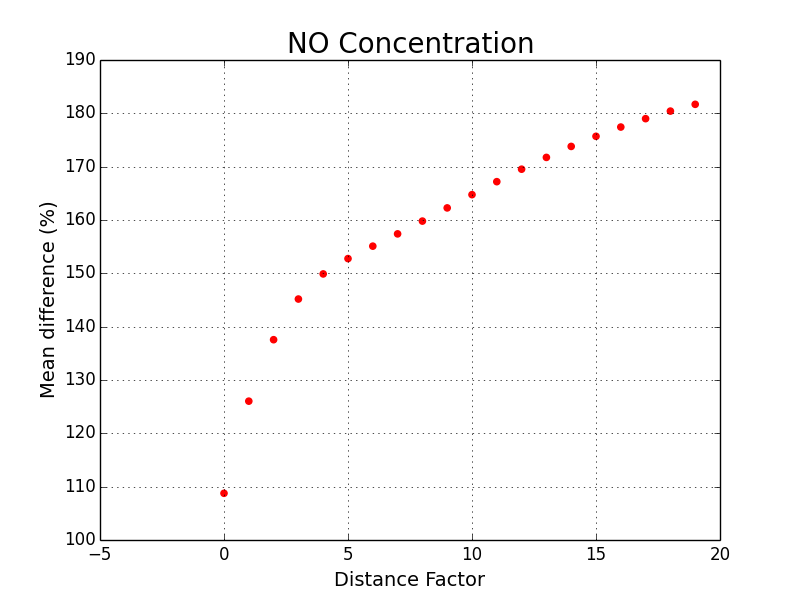
\includegraphics[width=\linewidth]{./images/IDW_P_NO.png}
                    \caption{}
                    \label{fig:idw_power_NO}
                \end{subfigure}
                \begin{subfigure}{0.6\textwidth}
                    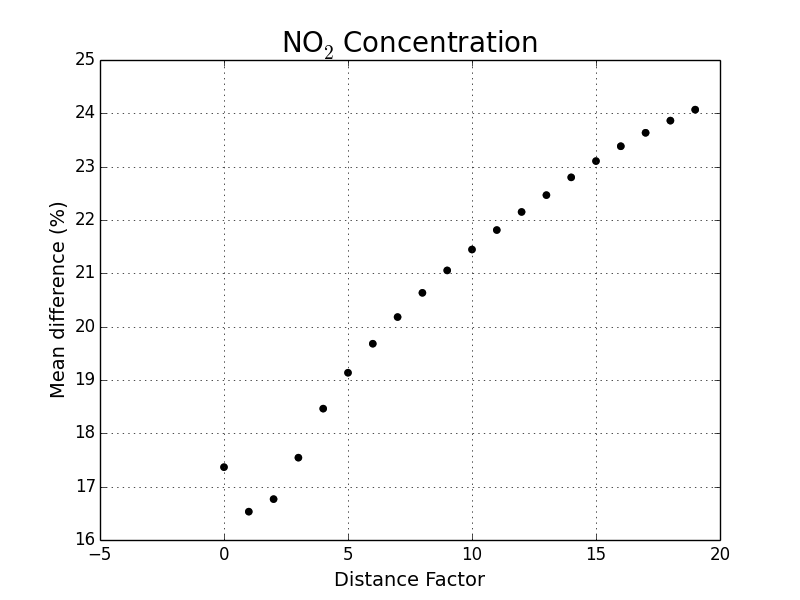
\includegraphics[width=\linewidth]{./images/IDW_P_NO2.png}
                    \caption{}
                    \label{fig:idw_power_NO2}
                \end{subfigure}
                \begin{subfigure}{0.6\textwidth}
                    \centering
                    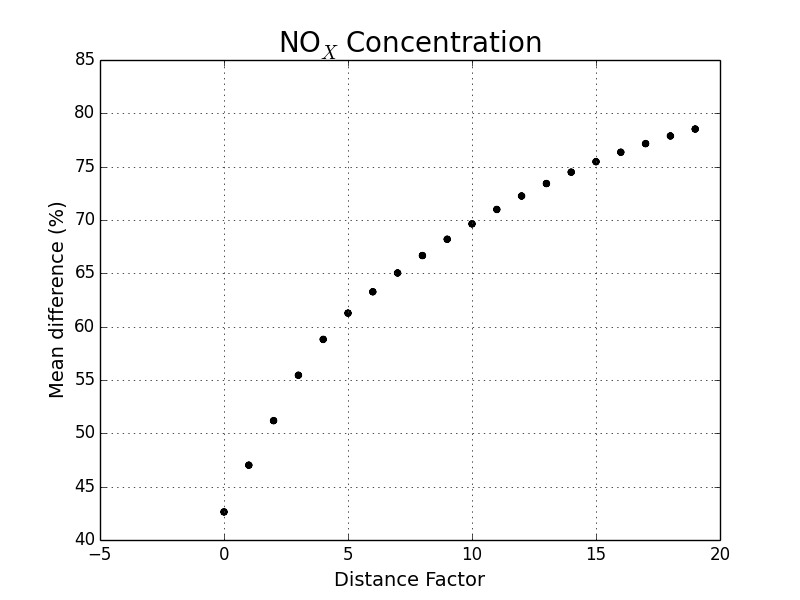
\includegraphics[width=\linewidth]{./images/IDW_P_NOx.png}
                    \caption{}
                    \label{fig:idw_power_NOx}
                \end{subfigure}
                \caption{These figures show how the optimal power parameter varies depending on the pollutant being measured.}
                \label{fig:idw_pollutant_compare}
            \end{figure}

            The minima seen in figure~\ref{fig:idw_power_all} is missing in two out of the three charts here. As such, the $NO_{2}$ reading is clearly dominating the others in the mean chart. From this it is clear that, at least for IDW, we must pay attention to all pollutants separately when testing with variable algorithm parameters. 

            If we run the tests once more, this time keeping pollutants separate, a very different picture is presented:

			\begin{table}[H]
				\centering
	    		\begin{tabular}{|c|c|c|}
	    			\hline
					Pollutant & Combined Mean Difference (\%) & Mean Difference (\%) \\ \hline
					$NO$ & 145.18 & 24.98 \\
					$NO_{2}$ & 17.54 & 7.59 \\
					$NO_{X}$ & 55.45 & 18.98 \\
					\hline
				\end{tabular}
				\caption{The mean results of IDW with the optimal power parameter for each pollutant.}
				\label{tab:idw_results_2}
			\end{table} 

			From table~\ref{tab:idw_results_2} we can see that having a power parameter specified for each pollutant is an extreme improvement on the overall performance of the algorithm. 

        \subsection{Bilinear}\label{prediction_evaluation_results_bilinear}

        	\centerimagewide{./images/Bilinear_Zurich.png}{The result of applying the bilinear algorithm to the data seen in figure~\ref{fig:zurich_ozone}.}{fig:bilinear_zurich}

        	With the bilinear interpolation algorithm, we have no optional parameters and the results are much simpler to calculate. We run the same tests, and average across all locations and time frames to get the results in table~\ref{tab:bilinear_results}.

        	\begin{table}[H]
				\centering
	    		\begin{tabular}{|c|c|}
	    			\hline
					Pollutant & Mean Difference (\%) \\ \hline
					$NO$ & 29.37 \\
					$NO_{2}$ & 5.08 \\
					$NO_{X}$ & 18.62 \\
					\hline
				\end{tabular}
				\caption{The mean results of bilinear interpolation.}
				\label{tab:bilinear_results}
			\end{table} 

        \subsection{Bicubic}\label{prediction_evaluation_results_bicubic}

        	\centerimagewide{./images/Bicubic_Zurich.png}{The result of applying the bicubic algorithm to the data seen in figure~\ref{fig:zurich_ozone}.}{fig:bicubic_zurich}

			As with the bilinear interpolation algorithm, we have no optional parameters in the bicubic interpolation algorithm and as such the results are simple to calculate. Again, running the same tests, and average across all locations and time frames to get the results in table~\ref{tab:bicubic_results}.

        	\begin{table}[H]
				\centering
	    		\begin{tabular}{|c|c|}
	    			\hline
					Pollutant & Mean Difference (\%) \\ \hline
					$NO$ & 18.38 \\
					$NO_{2}$ & 4.10 \\
					$NO_{X}$ & 11.22 \\
					\hline
				\end{tabular}
				\caption{The mean results of bicubic interpolation.}
				\label{tab:bicubic_results}
			\end{table} 

        \subsection{Natural Neighbour}\label{prediction_evaluation_results_natural_neighbour}

        	\tdi{I don't mention the convergence parameter}

        	\centerimagewide{./images/Natural_Neighbour_Zurich.png}{The result of applying the natural neighbour algorithm to the data seen in figure~\ref{fig:zurich_ozone}.}{fig:natural_neighbour_zurich}

        	Natural neighbour interpolation is also simple to get the results for. We use the same methodology as above to produce the results seen in table~\ref{tab:natural_neighbour_results}.

        	\begin{table}[H]
				\centering
	    		\begin{tabular}{|c|c|}
	    			\hline
					Pollutant & Mean Difference (\%) \\ \hline
					$NO$ & 25.37 \\
					$NO_{2}$ & 5.89 \\
					$NO_{X}$ & 16.84 \\
					\hline
				\end{tabular}
				\caption{The mean results of natural neighbour interpolation.}
				\label{tab:natural_neighbour_results}
			\end{table} 

        \subsection{Barnes}\label{prediction_evaluation_results_barnes}

        	\centerimagewide{./images/Barnes_Zurich.png}{The result of applying the nearest neighbour algorithm to the data seen in figure~\ref{fig:zurich_ozone}. This is the result of a single pass with a distance parameter of $2^{15}$.}{fig:barnes_zurich}

        	As with the nearest neighbour algorithm with Gaussian blurring and IDW, Barnes interpolation has parameters which need to be tuned in order to get the best performance. These parameters are the number of error correcting passes we make over the data, and the distance constant which we use to weight the values we use to interpolate. As we have seen in previous sections \todo{should this be plural?}, we should measure the result for each pollutant separately in order to achieve the best results. 

        	\centerimagewideanywhere{./images/Barnes_Mean_Difference_NO.png}{A scatter plot showing the difference for 23 different passes for each data time frame. The distance constant is 1024.}{fig:barnes_no_passes_results}

        	In order to determine the optimal number of passes for this algorithm we used the datasets. By running the algorithm with a varying number of passes, but with the same distance constant, in this case 1024, we can see how these subsequent passes alter the results. Figure~\ref{fig:barnes_no_passes_results} shows a scatter plot of the absolute percentage difference between the estimated value and the actual value. These results were calculated as the mean of the 3 usable data points in the Edinburgh data set. While we can see that there are differences depending on time, the relative difference between the initial calculation and the result after 24 passes is relatively constant. It should be point out at this time that, as discussed in section~\ref{background_interpolation_methods_barnes}, the greater the number of error correcting passes, the more the result converges to a single value. In the interest of calculation time the number of passes has been limited to 24. 

        	

        	As we can see, with no error correcting passes, we have a reasonable approximation of the result. The first subsequent pass corrects this error, however all subsequent passes do very little to improve the results. In the interest of computation time it would be reasonable to limit the number of passes to no more than five, however this only applies to a distance constant of 1024. In order to determine the changes for different distance factors a similar test to the above was run, with the number of passes remaining constant and the distance factor changing. The results of this test can be seen in figure~\ref{fig:barnes_distance_factor_results_NO}.

        	\centerimagewide{./images/Barnes_Distance_Factor_NO.png}{A scatter plot showing the error field difference for the ten different distance factors with the $NO$ pollutant.}{fig:barnes_distance_factor_results_NO}

        	From this graph it is clear that the greater the distance factor, the greater the difference successive passes make. This appears to continue until a distance of around $2^{17}$, which is also result with the lowest difference. At this point the difference made by applying many passes begins to decrease again. Furthermore we can see that the difference between passes decreases as the number of passes increases. As mentioned previously, due to computational time requirements these results were only calculated to 24 passes. However, increasing the runtime by 5 more passes, a run time increase of 20\% would only yield a potential accuracy increase of around a one hundredth of one percent. 

        	When we apply the same analysis to the pollutants $NO_{2}$ and $NO_{X}$, we get the results seen in figure~\ref{fig:barnes_distance_factor_results_NO2_NOx}. 

        	\begin{figure}[H]
                \centering
                \begin{subfigure}{\textwidth}
                    \centering
                    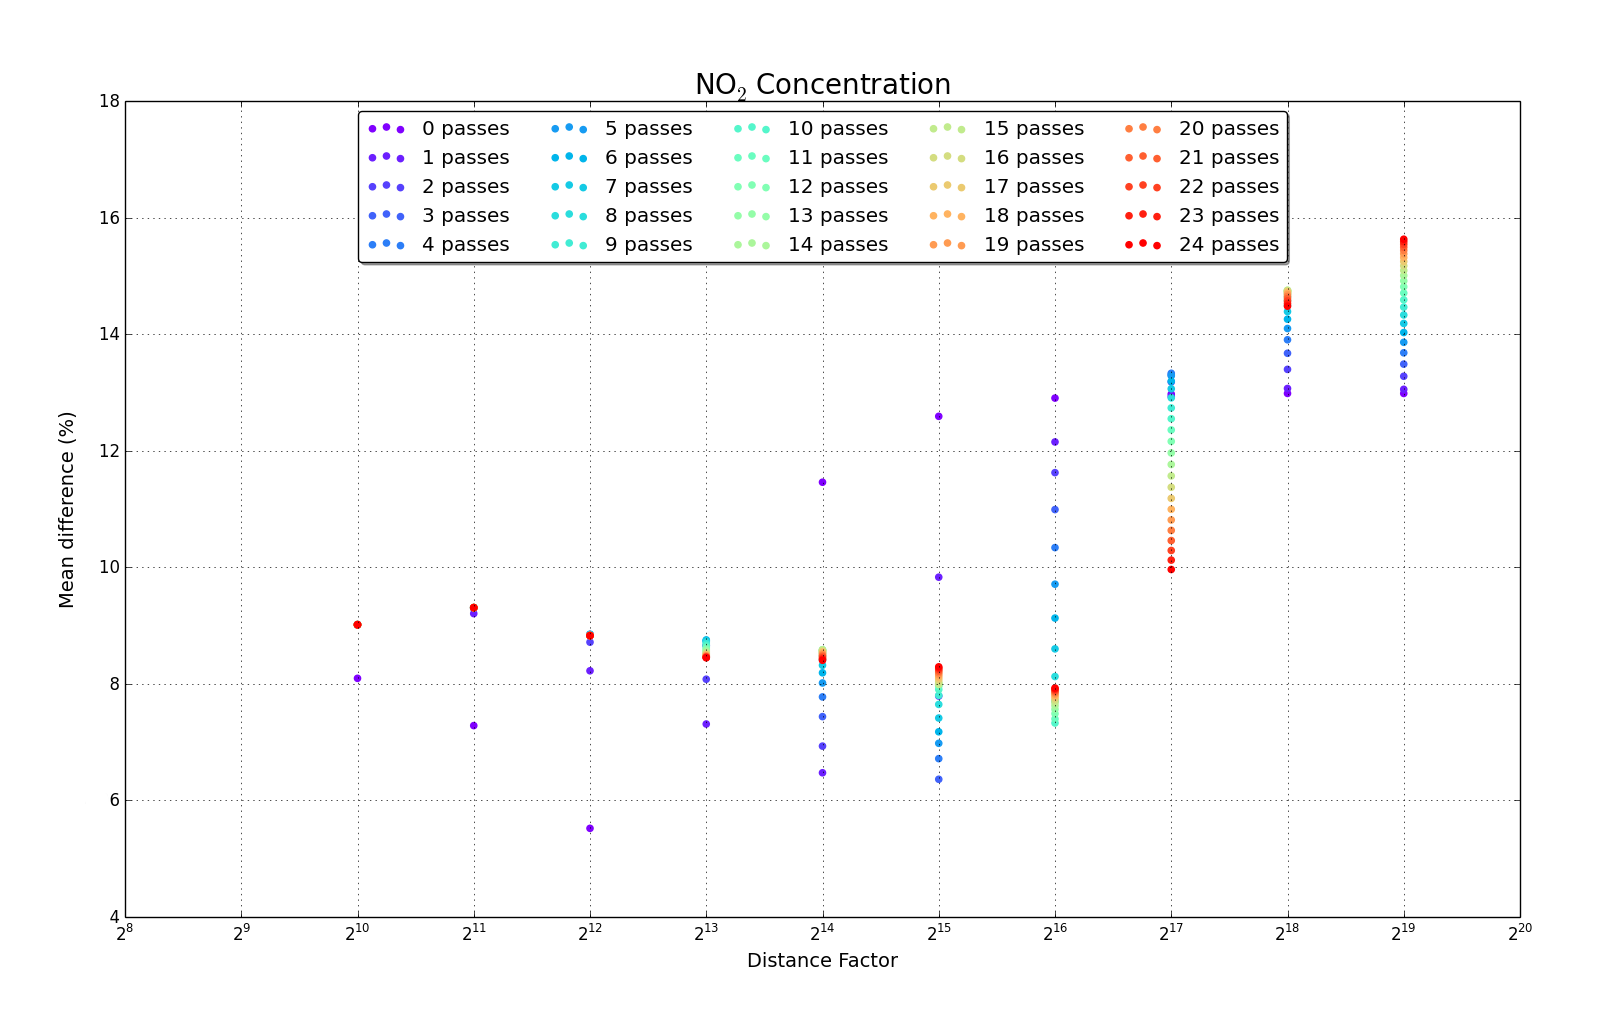
\includegraphics[width=\linewidth]{./images/Barnes_Distance_Factor_NO2.png}
                    \caption{Differences when applied to the $NO_{2}$ data in the Edinburgh data set.}
                    \label{fig:barnes_distance_factor_results_NO2}
                \end{subfigure}
                \begin{subfigure}{\textwidth}
                    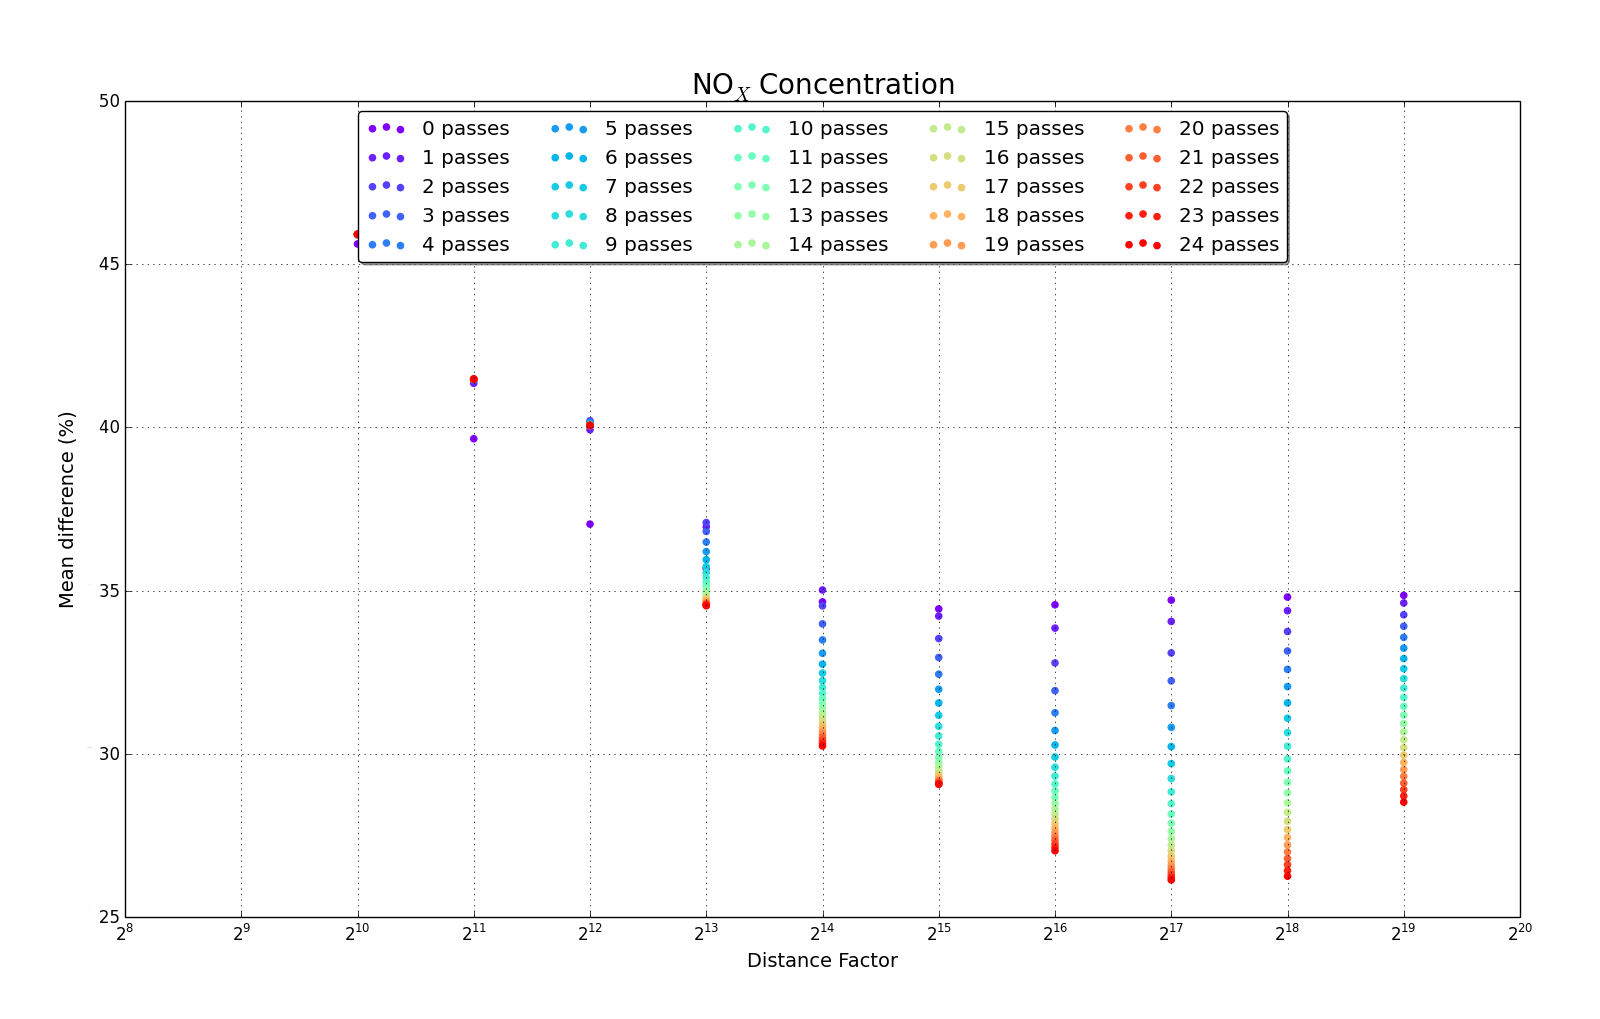
\includegraphics[width=\linewidth]{./images/Barnes_Distance_Factor_NOx.png}
                    \caption{Differences when applied to the $NO_{X}$ data in the Edinburgh data set.}
                    \label{fig:barnes_distance_factor_results_NOx}
                \end{subfigure}
                \caption{The difference between successive error correcting passes in Barnes interpolation when applied to the $NO_{2}$ and $NO_{X}$ data from the Edinburgh data set.}
                \label{fig:barnes_distance_factor_results_NO2_NOx}
            \end{figure}


        	The pollutants $NO$ and $NO_{X}$ appear to have the same tipping point in the distance factor, which is $2^{17}$. $NO_{2}$ is half of that distance at $2^{16}$. The graph also has a very different shape. 

        	With this new information of the distance factors and the optimal number of passes, that is to say for $NO$, $NO_{2}$ and $NO_{X}$ the distance factors are $2^{17}$,$2^{16}$ and $2^{17}$ respectively, we must run the tests once again. The results of these runs are seen in table~\ref{barnes_results}.

        	\begin{table}[H]
				\centering
	    		\begin{tabular}{|c|c|}
	    			\hline
					Pollutant & Mean Difference (\%) \\ \hline
					$NO$ & 15.73 \\
					$NO_{2}$ & 4.27 \\
					$NO_{X}$ & 10.33 \\
					\hline
				\end{tabular}
				\caption{The mean results of natural neighbour interpolation.}
				\label{tab:barnes_results}
			\end{table} 

		\subsection{Unexpected Results}

			When running these algorithms on the Edinburgh data set we get some unexpected results. As an example we will consider the bilinear interpolation algorithm compared to the nearest neighbour algorithm. Ordinarily we would expect nearest neighbour to perform the worse on our dataset as it does no interpolation between points at all. When we apply this algorithm to the Edinburgh data set we get a result like that seen in figure~\ref{fig:edinburgh_nearest_neighbour}. As we can see, applying the bilinear interpolation algorithm, as seen in figure~\ref{fig:edinburgh_bilinear}, we get a result with gradients between points which is what we would expect. It is unnatural for pollutant levels to change at some arbitrary boundary. 

			\begin{figure}[H]
                \centering
                \begin{subfigure}{0.7\textwidth}
                    \centering
                    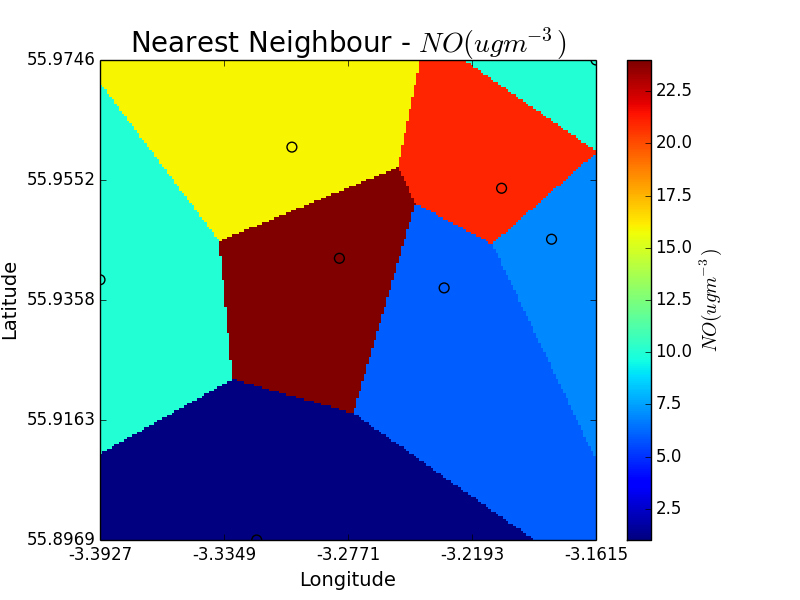
\includegraphics[width=\linewidth]{./images/Edinburgh_Nearest_Neighbour.png}
                    \caption{Nearest Neighbour}
                    \label{fig:edinburgh_nearest_neighbour}
                \end{subfigure}
                \begin{subfigure}{0.7\textwidth}
                    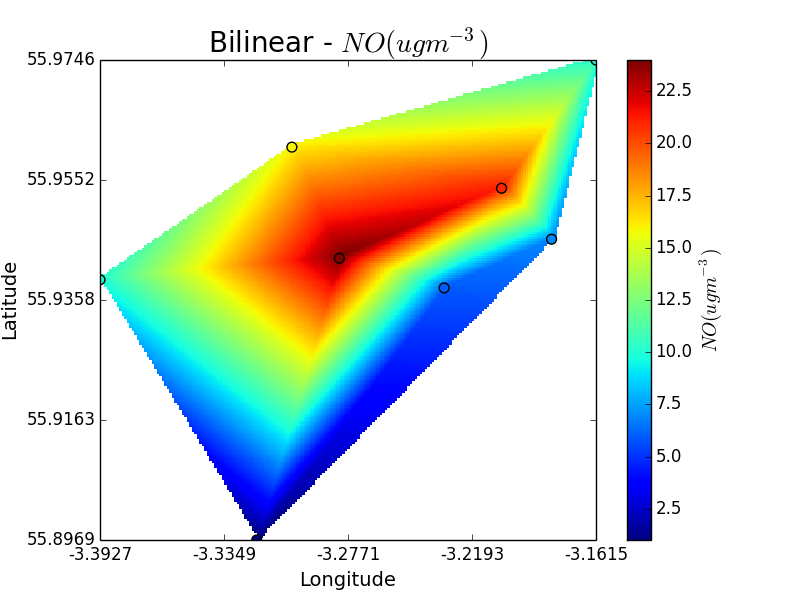
\includegraphics[width=\linewidth]{./images/Edinburgh_Bilinear.png}
                    \caption{Bilinear}
                    \label{fig:edinburgh_bilinear}
                \end{subfigure}
                \caption{The results of applying interpolation algorithms to all points in the Edinburgh data set.}
                \label{fig:edinburgh_example}
            \end{figure}

            Our data set also shows interesting characteristics as mentioned in section~\ref{prediction_evaluation_methodology_data_sets_air_quality_scotland}. One of the points in particular, the one closest to the centre of the image, has a much higher value than the surrounding points. This applies across all time frames and all pollutants. The reason for this is that the sensor is located next to a rather busy intersection and the others are not. As has been stated previously in this report, advanced interpolation models such as LUR would take this information into account. Our simple models cannot do this. Should we remove this point and create similar graphs to the above using nearest neighbour and bilinear interpolation the results are as follows:

            \begin{figure}[H]
                \centering
                \begin{subfigure}{0.7\textwidth}
                    \centering
                    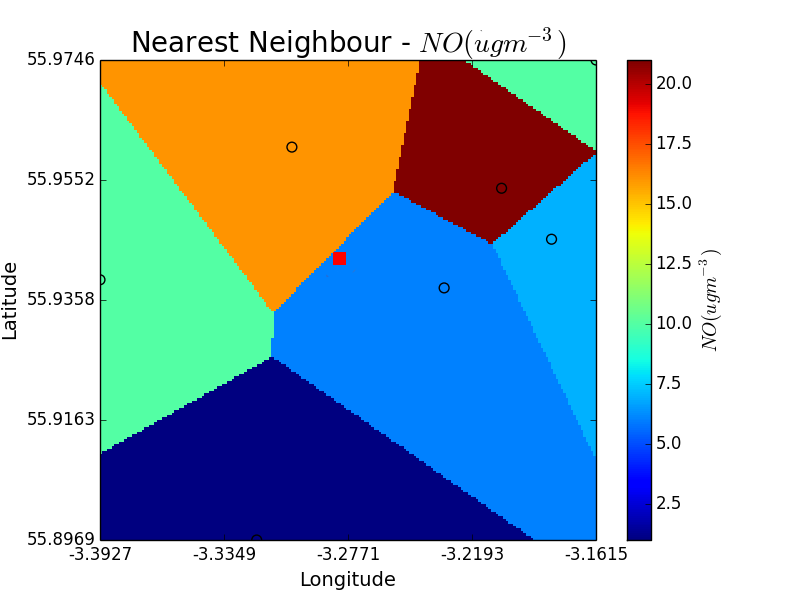
\includegraphics[width=\linewidth]{./images/Edinburgh_Removed_Nearest_Neighbour.png}
                    \caption{Nearest Neighbour}
                    \label{fig:edinburgh_removed_nearest_neighbour}
                \end{subfigure}
                \begin{subfigure}{0.7\textwidth}
                    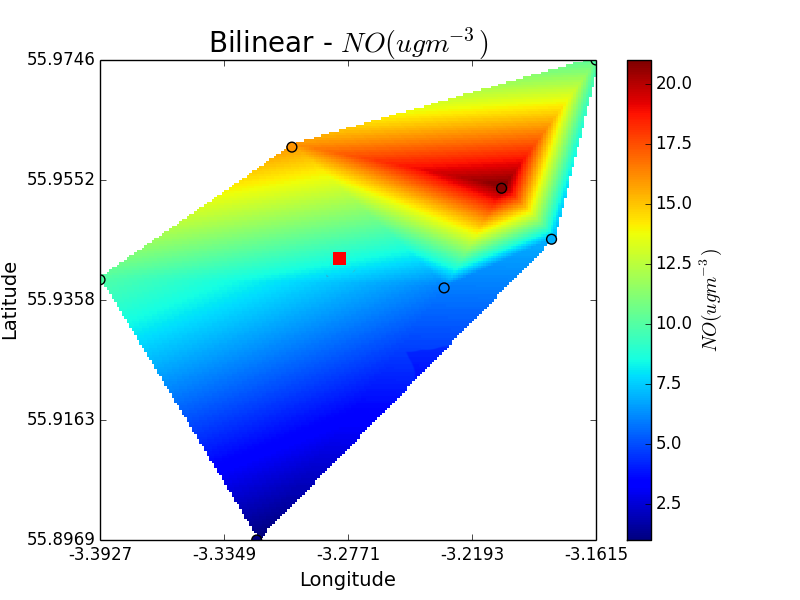
\includegraphics[width=\linewidth]{./images/Edinburgh_Removed_Bilinear.png}
                    \caption{Bilinear}
                    \label{fig:edinburgh_removed_bilinear}
                \end{subfigure}
                \caption{The results of applying interpolation algorithms to all points in the Edinburgh data set.}
                \label{fig:edinburgh_removed_example}
            \end{figure}

            The value at the removed point was 23.92$\mu gm^{-3}$, and this point has been marked as a red square on each of the maps. It should be noted that the colour scale has changed slightly as this point had this highest value, however the results are still obvious. In figure~\ref{fig:edinburgh_removed_bilinear} we can see that the value has been interpolated to a result similar to the light blue point at approximately -3.18,55.94. However, in figure~\ref{fig:edinburgh_removed_nearest_neighbour} which uses the nearest neighbour, it has interpolated to the slightly darker blue point at approximately -3.22,55.94. This result is closer to our original value. Due to the fact that with bilinear interpolation we can get gradients we would expect the bilinear algorithm to give the better result on average, however this is not the case as shown by the above example. The reasons for this are the lack of data points in the data set. If we were to have a higher number of data points, nearest neighbour would be more accurate, but more importantly, the bilinear algorithm would perform better. Missing out a single data point changed the view completely. With more data points, the effect that a single data point has is less and less pronounced. By having smooth gradients between these points we are more likely to predict the true values of unknown data points. With the small number we have, it is reduced to a probability calculation. 


	\section{Conclusion}

		\tdi{Talk more about being able to control parameters for different pollutants}

		One of the most important observations from section~\ref{prediction_evaluation_results} is the fact that tuning parameters to different pollutants can produce dramatically different results. Being able to control the distance parameter in IDW for example, increase the accuracy measurement almost 6 fold for one of the pollutants. Due to this we can propose the view that algorithms which give us control over parameters will generally out perform those where we cannot control the parameters. Applying a Gaussian blur algorithm to the nearest neighbour algorithm was hoped to prove this. It was shown in figure~\ref{fig:example_nearest_neighbour} that nearest neighbour with a Gaussian blur approximates bicubic interpolation. As we will show below, bicubic interpolation was one of the best contenders. However nearest neighbour, with Gaussian blur, did not perform as hoped, and in fact was the worst of the algorithms tested. Due to the data set, it is not believed that this result shows the failure of an algorithm with variable parameters out performing a similar algorithm with no parameters. Instead it is believed that we do not have enough data yet to prove in general this it is the case. Further experimentation is necessary to confirm this. 

		In terms of the relative performance of the algorithms the results are as follows:

		\begin{table}[H]
			\centering
    		\begin{tabularx}{\linewidth}{|X|X|X|X|X|X|X|X|}
    			\hline
				Pollutant & Nearest Neighbour & Blurred Neighbour & IDW & Bilinear & Bicubic & Natural Neighbour & Barnes \\ \hline
				$NO$ & 23.87\% & 24.52\% & 24.98\% & 29.37\% & 18.38\% & 25.37\% & 15.73\% \\
				$NO_{2}$ & 3.75\% & 13.05\% & 7.59\% & 5.08\% & 4.10\% & 5.89\% & 4.27\% \\
				$NO_{X}$ & 13.49\% & 18.99\% & 18.98\% & 18.62\% & 11.22\% & 16.84\% & 10.33\% \\
				\hline
			\end{tabularx}
			\caption{The mean results of various interpolation method.}
			\label{tab:all_results}
		\end{table}

		Alone this data provides very little information, as we have no way of comparing algorithms should one be better at a particular pollutant than the other. As such, we can create a table with the normalised difference percentages across pollutants. 

		\begin{table}[H]
			\centering
    		\begin{tabularx}{\linewidth}{|X|X|X|X|X|X|X|X|}
    			\hline
				Pollutant & Nearest Neighbour & Blurred Neighbour & IDW & Bilinear & Bicubic & Natural Neighbour & Barnes \\ \hline
				$NO$ & 0.14714 & 0.15113 & 0.15398 & 0.18105 & 0.11328 & 0.15642 & 0.09700 \\
				$NO_{2}$ & 0.08571 & 0.29845 & 0.17360 & 0.11613 & 0.09370 & 0.13476 & 0.09764\\
				$NO_{X}$ & 0.12434 & 0.17507 & 0.17504 & 0.17164 & 0.10345 & 0.15525 & 0.09521 \\ \hline
				Mean & 0.11906 & 0.20822 & 0.16754 & 0.15627 & 0.10348 & 0.14881 & 0.09662 \\
				\hline
			\end{tabularx}
			\caption{The relative performance of the interpolation methods.}
			\label{tab:all_ratio_results}
		\end{table}

		\centerimagewide{./images/Algorithm_Performance_Ratio.png}{The relative performance of the interpolation methods.}{fig:all_ratio_results}

		Table~\ref{tab:all_ratio_results} and figure~\ref{fig:all_ratio_results} show the results much more cleanly. By using the mean of these normalised results we can see that our best performing algorithm, for the Edinburgh data set is the Barnes algorithm. This result is followed closely by the bicubic algorithm and then nearest neighbour. These results are not representative however of a data set which would be returned  by a physical implementation of the sensors on buses and therefore cannot be used to show utility. Furthermore, due to the low number of data points, we cannot confirm that the comparisons of these algorithms for pollutant data is correct with any high degree of certainty. We can however state that it is likely that Barnes interpolation would perform the best given that research indicated its accuracy in these applications. Barnes interpolation is also the slowest method of interpolation unfortunately. As such it may be wise to use a slightly faster algorithm in a real world approach. Without a better data set, it is difficult to say which of the algorithms this would be. 

